\documentclass[12pt,fleqn]{article}\usepackage{../../common}
\begin{document}
Materyel Mekaniği - 6

Dönüş Mekaniği

Alttaki gibi bir kiriş düşünelim,

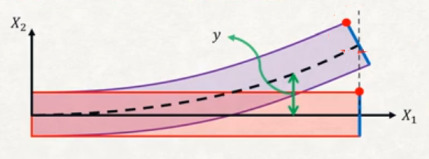
\includegraphics[width=20em]{phy_020_strs_06_01.jpg}

Daha önce bu tür bir kiriş üzerinde eksenel yöndeki kuvvetler ve yer
değişimlerinin ilişkisini

$$
\left[\begin{array}{c}
f'_{1x} \\ f'_{2x}
\end{array}\right] =
\frac{AE}{L}
\left[\begin{array}{cc}
1 & -1 \\ -1 & 1
\end{array}\right]
\left[\begin{array}{c}
u'_1 \\ u'_2
\end{array}\right]
\mlabel{1}
$$

olarak göstermiştik. Üstte yazılan kirişin yerel, kendisine has kordinat
sistemini baz alıyor. Eğer üstteki değişkenleri global kordinat sistemine
eşlemek, yansıtmak istiyorsak o zaman sistemi görülen $\theta$ kadar döndürmemiz
gerekiyor. Döndürme işlemi genel olarak iki boyuttaki bir $[u, v]$ vektörü için
[1, sf. 85]

$$
\left[\begin{array}{c}
u' \\ v'
\end{array}\right] =
\left[\begin{array}{cc}
C & S \\ -S & C
\end{array}\right]
\left[\begin{array}{c}
u \\ v
\end{array}\right]
\mlabel{2}
$$

ile yapılır, ki $C = \cos\theta$, $S = \sin\theta$.

Fakat unutmayalım tek eksenlikten çıktığımız zaman kirişin her ucunda iki
serbestlik derecesi vardır, her uç $u,v$ yönünde yer değişim yaşayabilir,
bunları $u_1,v_1$ ve $u_2,v_2$ diye gösterebiliriz. O zaman dönüş hesabı

$$
\left[\begin{array}{c}
u'_1 \\ v'_1 \\ u'_2 \\ v'_2
\end{array}\right] =
\left[\begin{array}{cccc}
C & S & 0 & 0 \\
-S & C & 0 & 0 \\
0 & 0 & C & S \\
0 & 0 & -S & C 
\end{array}\right]
\left[\begin{array}{c}
u_1 \\ v_1 \\ u_2 \\ v_2
\end{array}\right]
$$

Üstteki hesabı (1) formülü ile birleştirirsek, genişletilmiş (1) formu şu hale
gelir,

$$
\left[\begin{array}{c}
f'_{1x} \\ f'_{1y} \\ f'_{2x} \\ f'_{2y} 
\end{array}\right] =
\frac{AE}{L}
\left[\begin{array}{cccc}
1 & 0 & -1 & 0 \\
0 & 0 & 0 & 0 \\
-1 & 0 & 1 & 0 \\
0 & 0 & 0 & 0
\end{array}\right]
\left[\begin{array}{c}
u_1 \\ v_1 \\ u_2 \\ v_2
\end{array}\right]
$$

İlerlemeden önce iki üstteki dönüş matrisi, $T$ diyelim, hakkında ilginç bir
ispatı verelim, ileride lazım olacak. Acaba $T^T = T^{-1}$ ifadesi doğru mudur?
Bu aynı zamanda [1] kitabındaki 3.28 probleminin de cevabı. İspat için $T T^T$
çarpımını yapabiliriz, eğer birim (identity) matrisi elde edersek ispat tamam
demektir.

$$
T = 
\left[\begin{array}{cccc}
C & S & 0 & 0 \\
-S & C & 0 & 0 \\
0 & 0 & C & S \\
0 & 0 & -S & C 
\end{array}\right], \quad
T^T = 
\left[\begin{array}{cccc}
C & -S & 0 & 0 \\
S & C & 0 & 0 \\
0 & 0 & C & -S \\
0 & 0 & S & C 
\end{array}\right]
$$

Çarpımı \verb!sympy! ile yapalım,

\begin{minted}[fontsize=\footnotesize]{python}
from sympy import symbols, pprint, latex
from sympy.matrices import Matrix
C,S = symbols("C,S")
T = Matrix([[C,S,0,0],[-S,C,0,0],[0,0,C,S],[0,0,-S,C]])
Tprime = Matrix([[C,-S,0,0],[S,C,0,0],[0,0,C,-S],[0,0,S,C]])
print (latex(T * Tprime))
\end{minted}

\begin{verbatim}
\left[\begin{matrix}C^{2} + S^{2} & 0 & 0 & 0\\0 & C^{2} + S^{2} & 0 & 0\\0 & 0 & C^{2} + S^{2} & 0\\0 & 0 & 0 & C^{2} + S^{2}\end{matrix}\right]
\end{verbatim}

\LaTeX\quad ile

$$
\left[\begin{matrix}C^{2} + S^{2} & 0 & 0 & 0\\0 & C^{2} + S^{2} & 0 & 0\\0 & 0 & C^{2} + S^{2} & 0\\0 & 0 & 0 & C^{2} + S^{2}\end{matrix}\right]
$$

Hatırlarsak $C = \cos\theta, S = \sin\theta$, bunları yerine koyunca tüm köşegen
boyunca 1 değeri elde edilir, diğer hücrelerde sıfır var, demek ki bir birim
matrisi elde ettik. Bu demektir ki $T T^T = I$, ve bu ifadenin doğru olmasının
tek yolu $T^T = T^{-1}$ olmasıdır.

Dönüş mekaniğini gördük, şimdi önceki derste işlenen kiriş parçasına hem
eksenel dinamiği hem de biraz önce gördüğümüz dönüş mantığını ekleyelim.
Altta görülen kiriş parçasının hareketlerini hesaplayabilmek istiyoruz yani,

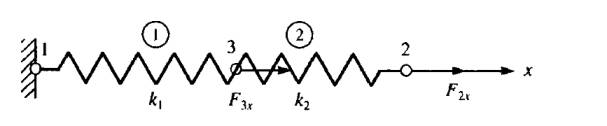
\includegraphics[width=15em]{phy_020_strs_06_02.jpg}

Önceki dersten hatırlarsak eksene dik parçaların mekaniği alttaki formülle
gösterilmişti,

$$
\left[\begin{array}{c}
f_{1y} \\ m_1 \\ f_{2y} \\ m_2
\end{array}\right] =
\frac{EI}{L^3}
\left[\begin{array}{cccc}
12 & 6L & -12 & 6L \\
6L & 4L^2 & -6L & -6L \\
-12 & -6L & 12 & -6L \\
6L & 2L^2 & -6L & 4L^2
\end{array}\right]
\left[\begin{array}{ccc}
v_1 \\ \phi_1 \\ v_2 \\ \phi_2
\end{array}\right]
$$

Bu formüle (1)'deki eksenel mantığı eklersek, yerel kordinatlarda

$$
\left[\begin{array}{c}
f'_{1x} \\ f'_{1y} \\ m'_1 \\ f'_{2x} \\ f'_{2y} \\ m'_2
\end{array}\right] =
\left[\begin{array}{cccccc}
C_1 & 0 & 0 & -C_1 & 0 & 0 \\
0 & 12C_2 & 6 C_2 L & 0 & -12 C_2 & 6 C_2 L \\
0 & 6C_2 L & 4 C_2 L^2 & 0 & -6 C_2 L & 2 C_2 L^2 \\
-C_1 & 0 & 0 & C_1 & 0 & 0 \\
0 & -12C_2 & -6 C_2 L & 0 & 12 C_2 & -6 C_2 L \\
0 & 6 C_2 L & 2 C_2 L^2 & 0 & -6C_2 L & 4C_2 L^2
\end{array}\right]
\left[\begin{array}{c}
u'_1 \\ v'_1 \\ \phi'_1 \\ u'_2 \\ v'_2 \\ \phi'_2
\end{array}\right]
$$

elde edilir, ki $C_1 = \dfrac{AE}{L}$ ve $C_2 = \dfrac{EI}{L^3}$
olmak üzere. 


[devam edecek]

Kaynaklar

[1] Logan, {\em A First Course in the Finite Element Method, 6th Ed}

\end{document}
